\chapter{基于工具图谱与深度优先遍历的工具编排与调用方法}

\section{引言}
\label{sec:intro}

\indent 在第三章中,我们介绍了基于工具调用路径构建的工具知识图谱,包括有对调用路径数据的清洗、工具图谱的构建方法、工具节点召回模型训练等部分。
尽管工具图谱能够表示大量的工具调用路径,
但是仅依赖图上搜到的路径不具有灵活性,图上固有的路径不能满足变化的用户需求。
同时,工具也具有生命周期和动态性,会有新建的工具或者废弃的工具,图谱上的节点也会随之变化,
因此需要一种动态的工具选择方法。
使用大语言模型进行选择和编排能够提升系统的动态性和灵活性,但仅依赖大语言模型的语义分析能力难以处理工具之间的复杂依赖关系。

因此,我们提出了一个在工具图谱上动态遍历的算法,通过大语言模型智能体在图上动态选择节点。本章集中介绍图谱遍历和工具路径选择的部分,即如何根据用户需求在大型工具图谱上进行高效的搜索和选择。
在本章主要有以下几个重要问题需要研究:
1.如何合理利用工具图谱上的依赖信息进行工具选择?
2.如何对路径选择流程进行优化,以提升整体的准确率和效率?
3.如何处理工具调用中遇到的工具调用异常、工具响应过长等问题?

\indent 针对上述问题,我们提出了一种基于工具图谱的动态寻路算法。该算法首先将用户的需求进行分析和拆解,以得到
更小的任务编排与执行单位。其次,本章提出了一种基于深度优先搜索的搜索算法,
能够实时地在图上进行搜索并选择合适的工具调用路径。
最后,为了进一步精简返回结果内容、减少推理延迟和提升系统效率,
我们提出了一种响应压缩方法,通过让模型选择与用户需求有关的字段来生成压缩后的响应结果,
能够有效保留重要信息并提升交互效率。

\section{整体框架}

图~\ref{fig:ch4-framework}展示了本章提出的基于深度优先遍历算法的动态工具编排算法的整体技术框架。

\begin{figure}[!htp]
  \vspace{1em}
  \centering
  \setlength{\abovecaptionskip}{10pt} % 控制图片和caption之间的距离
  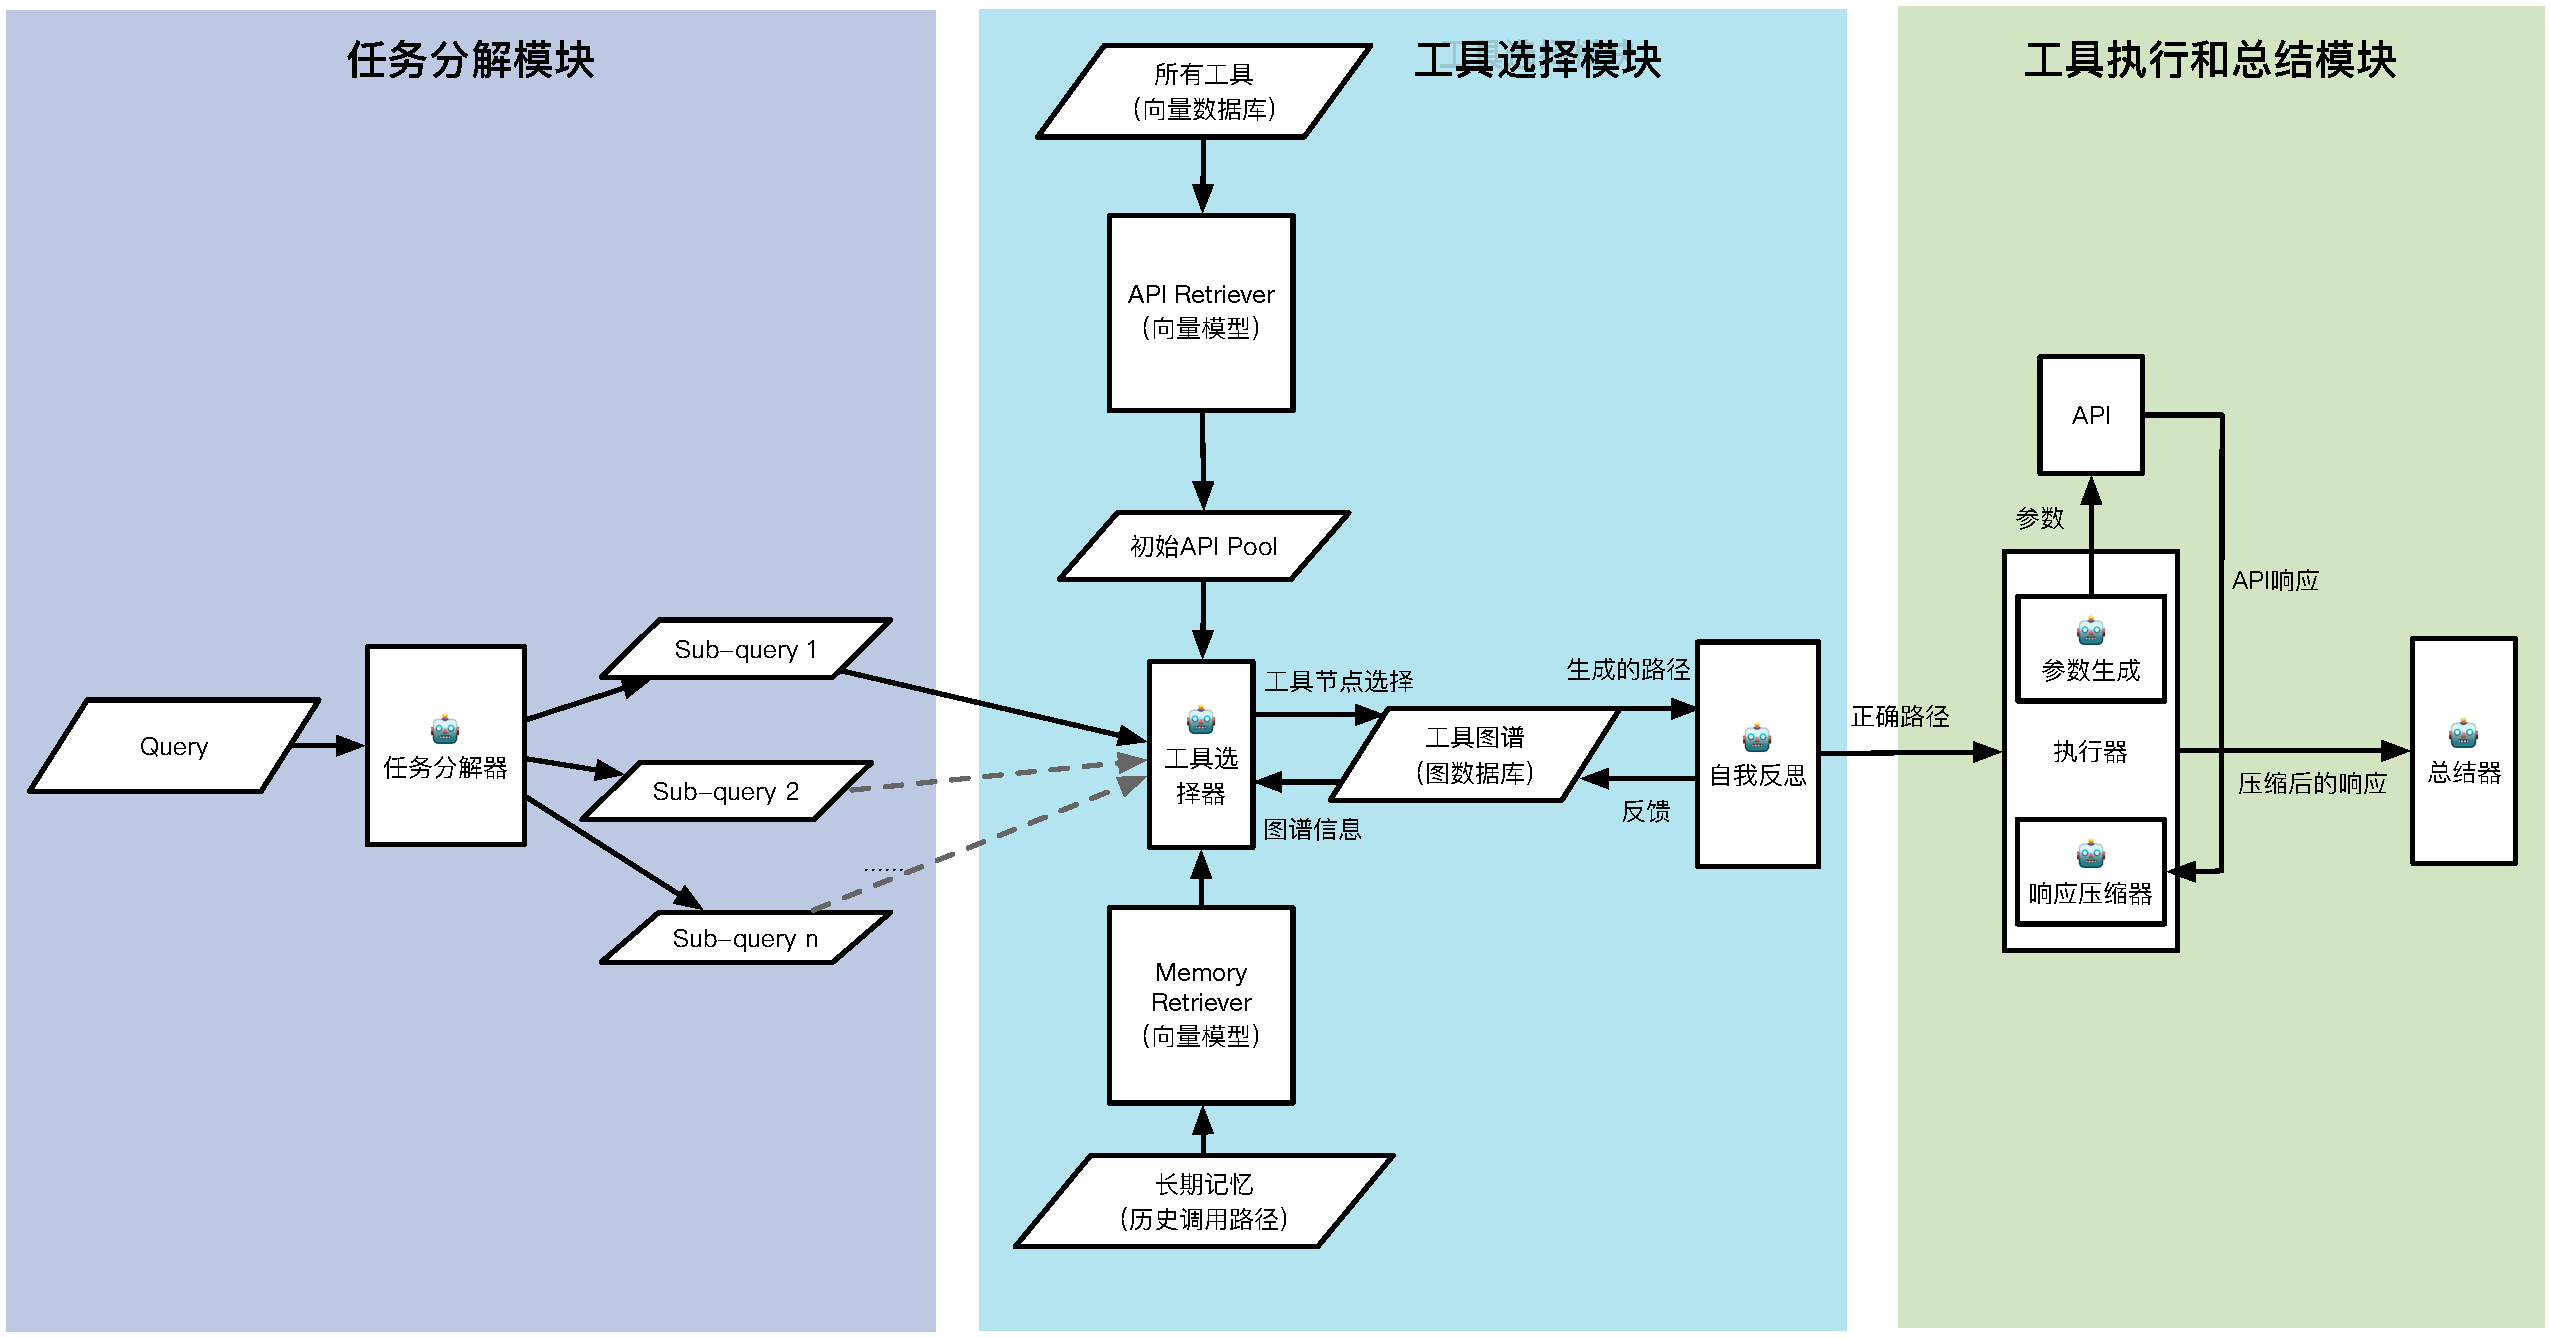
\includegraphics[height=7cm]{../assets/ch4-整体框架图-3.pdf}
  \bicaption{整体框架}{Overview of the Dynamic Tool Selection Framework}
  \label{fig:ch4-framework}
\end{figure}

该方法整体由以下几个部分组成:

\begin{enumerate}
  \item \textbf{任务分解模块}:任务分解模块通过对用户模糊或复杂需求进行解析,将其拆解为明确且独立的子任务,使复杂问题变得更易执行和解决。模块利用语义分析,根据任务的逻辑结构和类别对需求进行分解,既提升了任务处理的效率,也增强了系统的响应准确性。同时,通过识别任务间的依赖关系,确保了整体任务流程的有序性和可执行性。
  \item \textbf{工具选择与编排模块}:该部分包括基于深度优先遍历的动态工具搜索算法、自我反思机制和记忆模块。
  本质上来说,该算法就是在图上进行深度优先遍历,我们将图上的节点的权值、节点的邻居点的边权等信息,以及节点工具的描述信息等全部提供给大语言模型,让模型在图上动态选择节点。
  在工具路径选择的过程中,若遇到了路径信息,我们将会进调用“自我反思机制”,即对路径上遇到的错误进行分析并基于此错误分析内容重新
  进行路径选择。模型可以选择回溯到某个中间过程,或者是从头开始寻路。
  在大语言模型智能体不断寻路的过程中,我们会维护一个“短期记忆”,即对整体寻路流程的记录。
  为了利用历史经验知识,我们添加了“长期记忆模块”,即我们会搜索类似任务的历史工具调用路径放在提示词辅助大语言模型的规划。
  自我反思机制能够通过格式化的反思提升系统的准确性。
  \item \textbf{工具调用与总结模块}:在得到了整体的路径后,任务执行模块负责调用工具,并将结果进行汇总,最终输出结果。
  其中涉及到了工具参数配置、工具响应压缩模块。工具参数配置模块直接将工具的说明信息和所需参数信息提供给模型,让模型提供合适参数并进行校验。
  工具响应压缩模块则负责对工具的响应结果进行压缩,以减少响应时间,提升交互效率。我们将任务总结智能体作为一种
  特殊形式的工具,在所有前序工具执行结束后调用,针对用户需求输出最终结果。
\end{enumerate}

在流程上,对于每个用户需求,只会执行一次子任务分解。但是对于每个子任务,都会执行一次动态工具搜索算法,并且会根据搜索到的工具路径执行若干次工具,因此会多次调用工具执行模块。
最后,我们通过任务总结模块对所有子任务的结果进行汇总,得到最终输出。

\section{具体实现}

\subsection{任务分解模块}

由于用户的需求可能会较为模糊、笼统,或者在同一个需求语句中存在多个潜在的子任务。通过对用户提供的复杂需求进行分解、改写,并生成适合执行的具体指令,这一过程使得任务变得更加明确和易于解决。

任务分解模块的输入包括具体用户需求、子任务格式的指令、输出格式案例以及当前工具的具体分类,输出则是JSON格式的一组子任务。

每个子任务都是一个独立的执行单元,包括“子任务编号“、“子任务描述”、“子任务类别”等重要信息。
子任务之间可能会存在时间或者参数上的依赖,该依赖会在任务分解的时候通过特殊的占位符来表示,用于串联整体的任务编排流程。

首先,任务分解模块的核心功能是将用户提出的复杂或模糊需求拆解为可执行的子任务。
许多用户在表达需求时,往往由于信息不明确或需求过于笼统,
导致系统难以直接响应。
例如,用户可能提出多个相关或不相关的要求,或者在一个指令中混合了不同领域的子任务。
在这种情况下,大语言模型通过对用户输入的语义分析,将任务按照逻辑和类别进行分解。
逻辑上分解有利于明确每个任务的目标,没有依赖关系的任务可以并行执行,能够有效提高任务的效率和正确率。
按照类别来分解能够缩小在工具池中的搜索范围,提高搜索效率和准确性。
其提示词如下所示:

% Set Colors
\definecolor{bgcolor}{RGB}{240,240,240} % Background color
\definecolor{titlecolor}{RGB}{20,20,20} % Title background color

\begin{center}
% Create background with tcolorbox
\begin{tcolorbox}[colback=bgcolor, colframe=black, width=0.85\textwidth, boxrule=0.5mm, 
coltitle=white, colbacktitle=titlecolor, title=Task Decomposition and Response Planning with GPT-4]

% Centered content

\textbf{Instruction Prompt:} Decompose the task and plan its steps in a structured way. Identify tool dependencies and output the result as a JSON list.

\textbf{Task Description:}  
1. Break down the task into multiple subtasks in a step-by-step manner. Each subtask should be labeled as \textbf{StepX} (e.g., Step1, Step2).  
2. Specify tool usage and dependencies:  
   - If a step depends on another step's result, represent the input using its output reference, e.g., \texttt{Input: [A1]} where \texttt{A1} refers to the result from Step1.  
   - Use multiple inputs if needed, e.g., \texttt{Input: [A1, A3]}.  
3. Output the plan in a \texttt{JSON} format list.  
4. Ensure logical dependencies and a clear structure for each subtask. 

\textbf{Example Task:}  
What is the most popular travel destination in Europe? And what’s the weather like there?

\textbf{Expected Output:}  
\texttt{%
\{ \\
\ \ \ "Steps": [ \\
\ \ \ \ \ \ \ \{ "Step1": "Identify the most popular travel destination in Europe.", "context": [], "category": "travel" \}, \\
\ \ \ \ \ \ \ \{ "Step2": "Fetch the current weather for the identified destination.", "context": ["A1"], "category": "weather" \}, \\
\ \ \ \ \ \ \ \{ "Step3": "Generate a summarized response combining the destination and weather information.", "context": ["A1", "A2"], "category": "llm" \} \\
\ \ \ ]
\}
}

\end{tcolorbox}
\end{center}

通过以上的大语言模型提示词工程,我们可以让大语言模型输出JSON格式的任务执行流程,并且根据任务之间的依赖关系对任务进行排序。

如图\ref{fig:ch4-decomposition}最终形成的子任务图是一个有向无环图,其中每个节点代表一个子任务,每条边代表任务之间的依赖关系。

\begin{figure}[!htp]
  \vspace{1em}
  \centering
  \setlength{\abovecaptionskip}{10pt} % 控制图片和caption之间的距离
  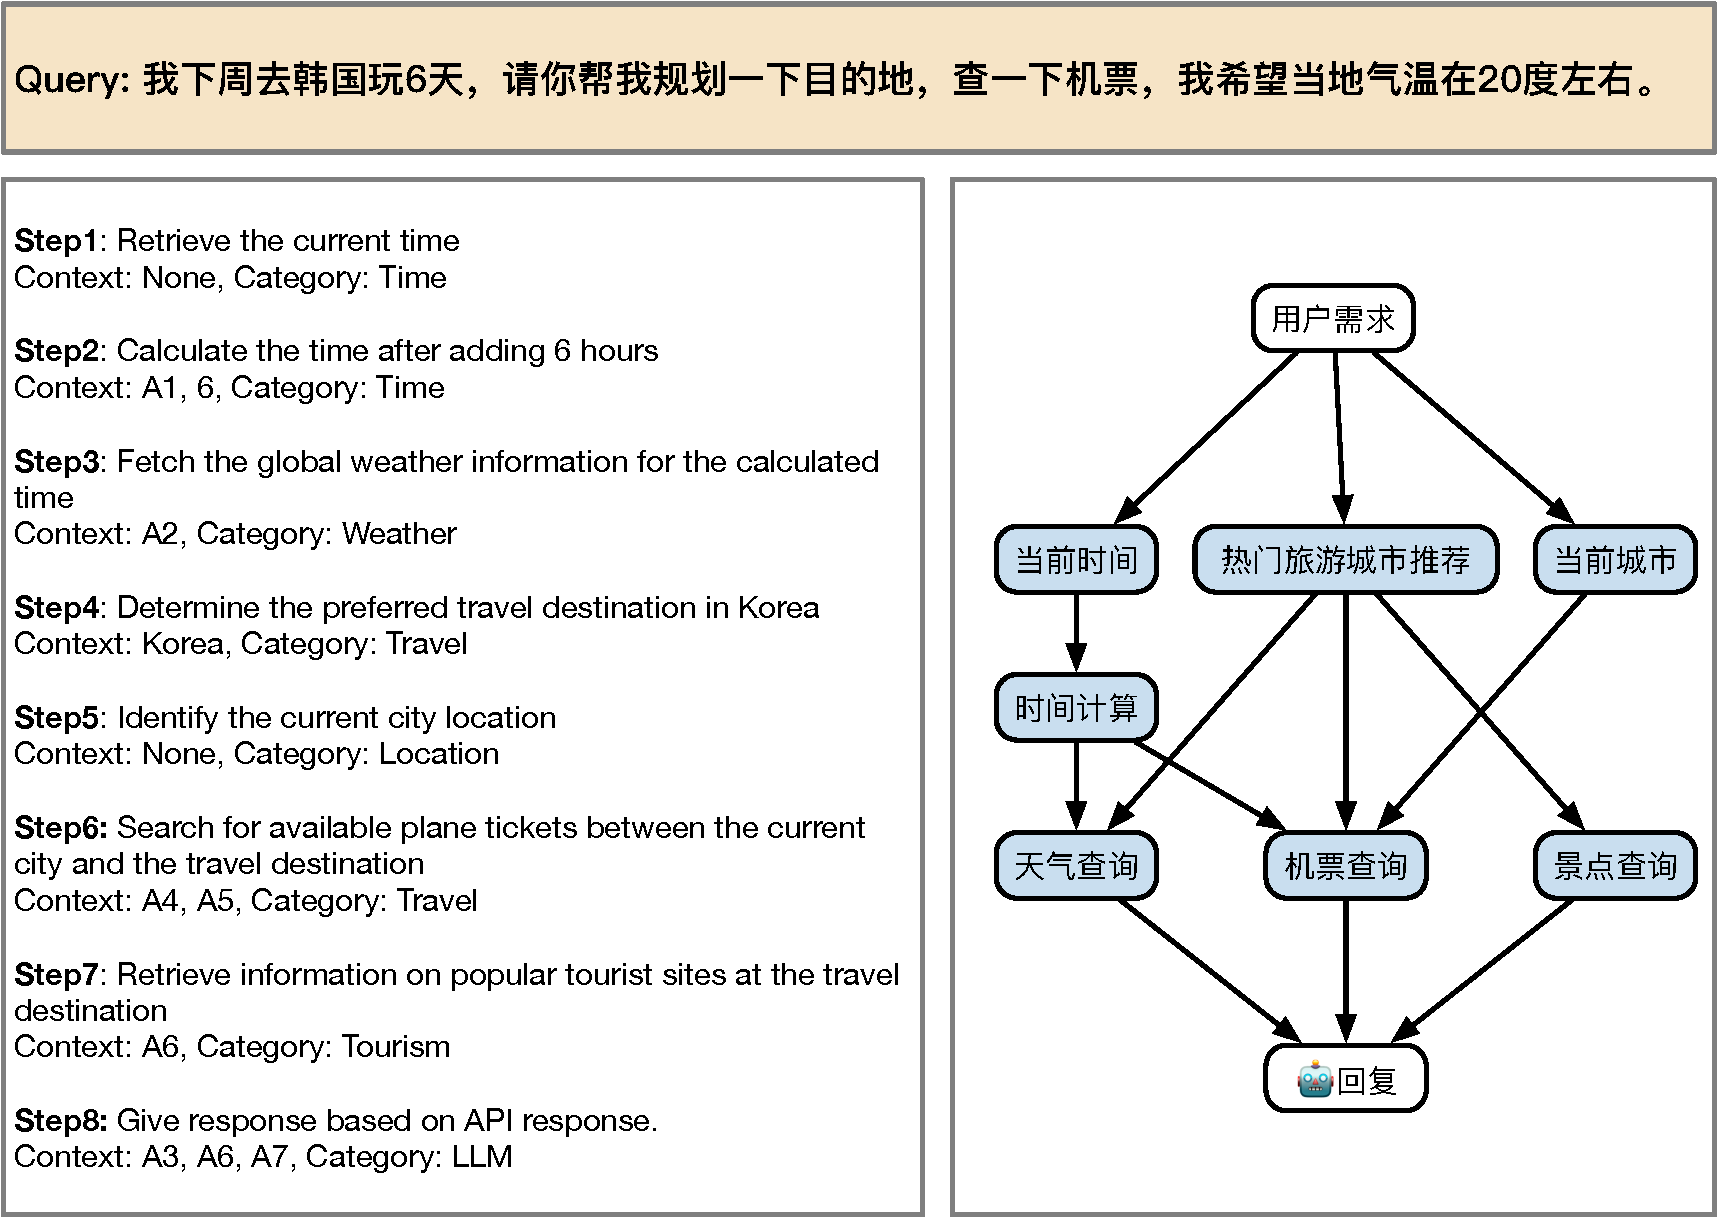
\includegraphics[height=7cm]{../assets/ch4-任务分解模块.pdf}
  \bicaption{任务分解模块}{Task Decomposition Module}
  \label{fig:ch4-decomposition}
\end{figure}

总的来说,基于大语言模型的任务分解模块通过分解复杂任务、改写用户需求,并显式表示子任务之间的依赖,使得该系统在执行复杂任务时更加灵活、精准且高效。

\subsection{工具选择与编排模块}

为了更好地利用我们构建的工具图谱,并挖掘隐藏节点关系中的知识,
我们开发了一个基于深度优先遍历的寻路算法。
与“思维链”(Chain-of-Thought)或ReACT方法相比,
该算法的优点在于该方法在图谱上进行可回溯的动态选路,能够防止错误传播的问题,
并能够对整个工具空间进行更全面的探索。
在动态选择工具路径的同时,我们会维护一个“短期记忆”,即
当前的路径和每一步路径选择(前进/回溯)的理由。同时,为了利用历史经验知识,
我们将历史上类似任务的正确工具路径作为提示词提供给模型,以辅助模型进行路径选择。
最后,在该算法能够通过“自我反思机制”来对路径进行判断和错误诊断,
这一机制进一步提升了路径选择的准确率。

\subsubsection{基于深度优先遍历的工具选择算法}

图~\ref{fig:ch4-dfs}为本文提出的工具选择算法的效果展示。

\begin{figure}[!htp]
  \vspace{1em}
  \centering
  \setlength{\abovecaptionskip}{10pt} % 控制图片和caption之间的距离
  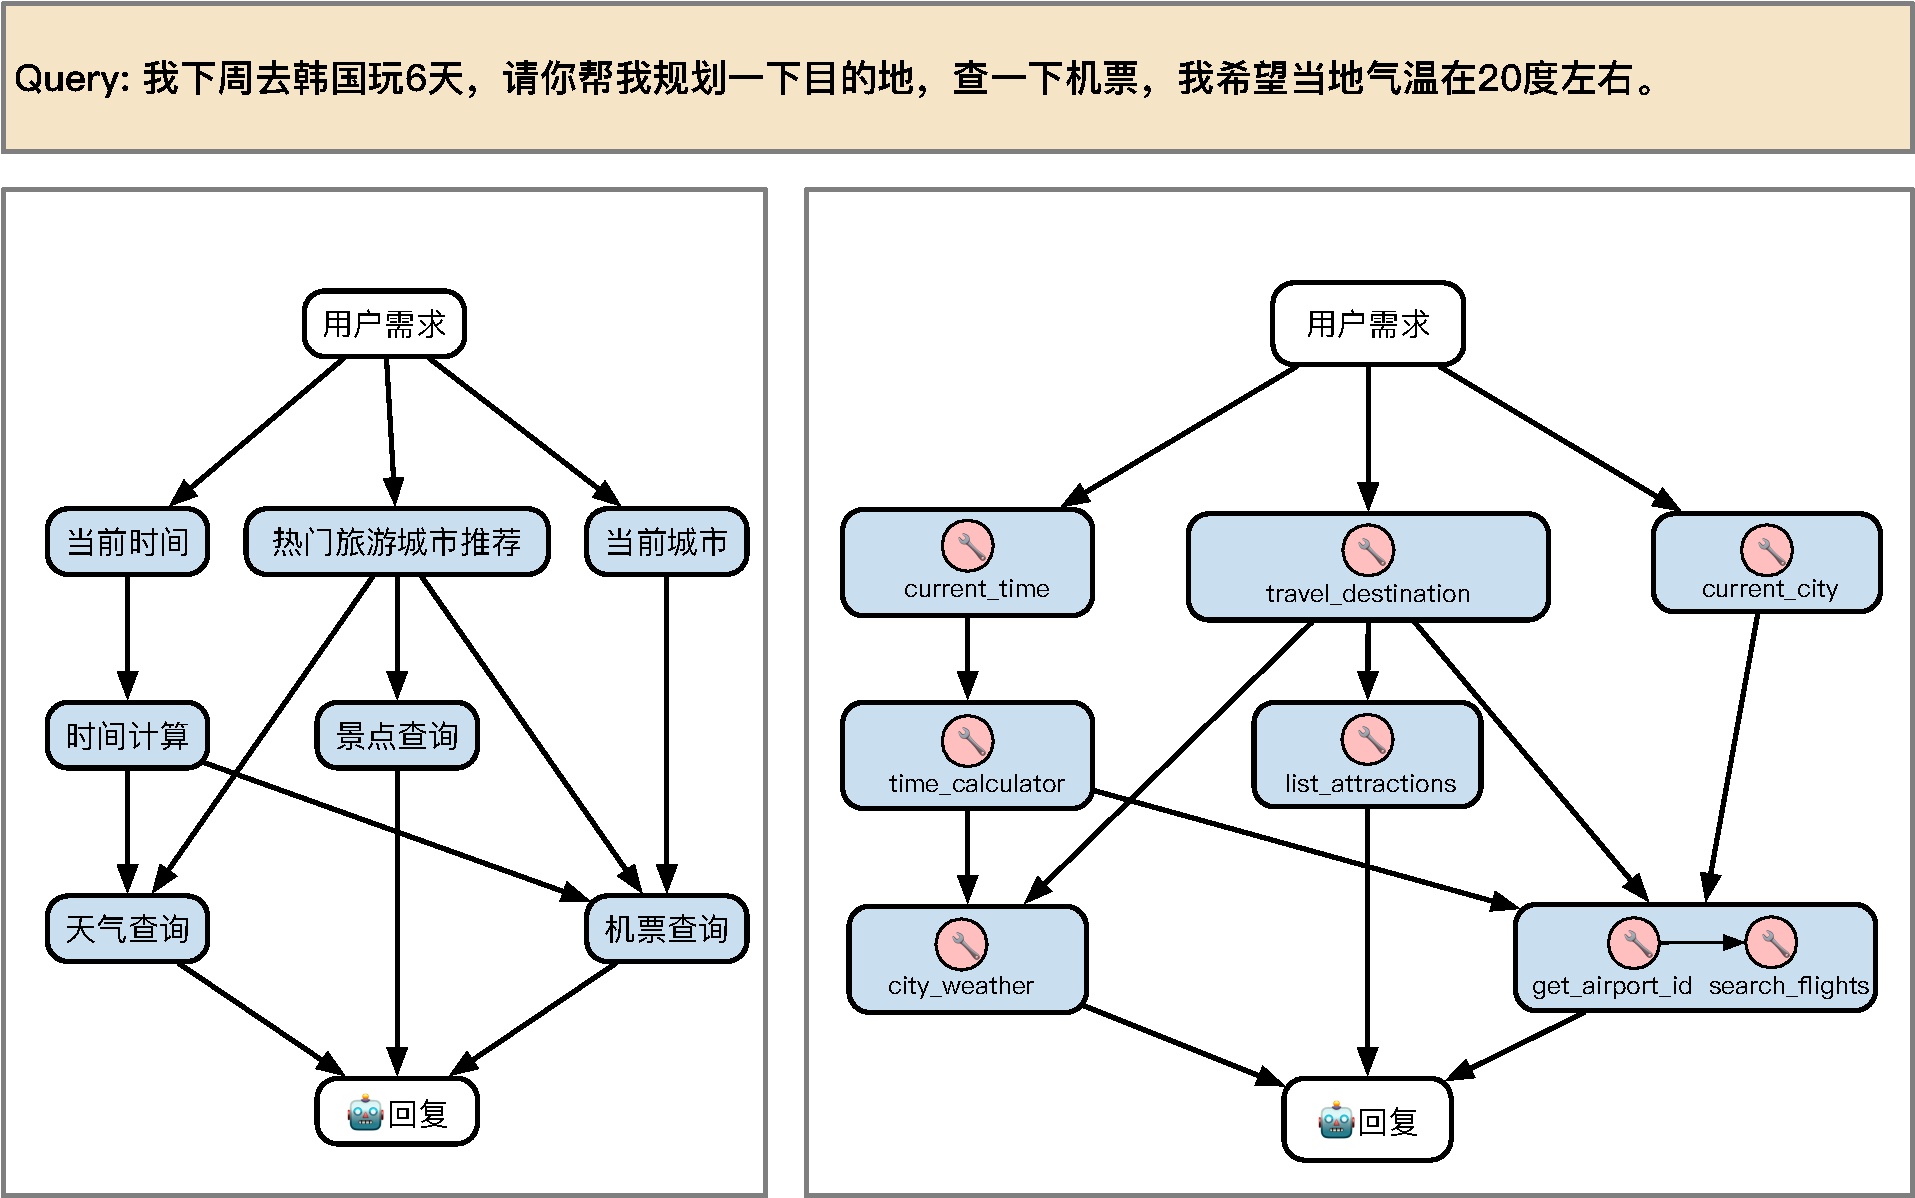
\includegraphics[height=8cm]{../assets/ch4-工具选择器.pdf}
  \bicaption{基于深度优先遍历的工具选择算法}{Dynamic Tool Selection based on DFS}
  \label{fig:ch4-dfs}
\end{figure}

首先,在上一步任务分解模块中,我们将整个任务构建为一个有向无环图,并且用边来表示任务之间的依赖关系。
那么我们在选择每个子任务的工具时,需要考虑到前序任务的所调用的工具。

因此算法流程如下所示,对没有前序任务的节点,我们通过语义相似度算法得到一组候选的工具集合,然后通过
提供LLM这些工具的名称、描述和参数等信息,直接让LLM来选择对应的工具。

对于有前序任务的节点,我们通过寻找前序任务的工具节点的邻居节点来得到一组候选工具。不同前序任务之间的邻居节点取并集提供给LLM。
在筛选邻居时,我们会根据任务分解器的“类别”字段筛选特定工具类别的邻居,以过滤掉噪声工具节点,提高工具选择的有效性。
若取并集之后的工具节点仍过多,我们将会计算每个工具与子任务描述的相似度,并进行排序,选择前K个工具节点提供给大语言模型。
我们设计了简单实验来选择这个K值以及选取前K个的有效性,具体见第五章的实验部分。

对于搜索得到的邻居节点,我们在提示词中对不同类别的依赖关系设置了不同程度的重要性,引导大语言模型选择合适的工具节点来完成子任务。

在处理具有前序任务的工具节点时,我们通过寻找这些工具节点的邻居节点生成候选工具集合。对于多个前序任务节点,其邻居节点取并集,形成综合依赖关系的候选工具集供大语言模型(LLM)使用。

为了提高工具选择的有效性,我们依据任务分解器的“类别”字段筛选相关工具节点,过滤掉与任务无关的噪声节点。如果候选工具仍然过多,则计算工具与子任务描述的语义相似度,并选择前 $K$ 个最相关的工具作为候选。

提示词中引入了依赖关系优先级规则,以引导大语言模型选择合适工具完成子任务。依赖关系的优先级为:强依赖 > 弱依赖 > 时序依赖。

以下为提示词示例:

\definecolor{bgcolor}{RGB}{240,240,240} % 背景颜色
\definecolor{titlecolor}{RGB}{20,20,20} % 标题背景颜色

\begin{center}
\begin{tcolorbox}[colback=bgcolor, colframe=black, width=0.85\textwidth, boxrule=0.5mm, coltitle=white, colbacktitle=titlecolor, title=Example Prompt for Tool Selection]

\textbf{Instructions:} You are tasked with selecting the most appropriate tools to solve the given sub-task. Based on the provided tool descriptions and their dependencies, choose tools in the following order of priority: \textbf{Strong dependency > Weak dependency > Sequential dependency}. Use the chosen tools to complete the sub-task.

\textbf{Sub-task:} Calculate the time difference between the current time and a target time.

\textbf{Available Tools:}
\begin{enumerate}
    \item \textit{Current Time Retrieval Tool:} No dependency, Time Information.
    \item \textit{Time Difference Calculator Tool:} Weak dependency (requires \texttt{current\_time} as input).
    \item \textit{Time Zone Converter Tool:} Sequential dependency (depends on output from Time Difference Calculator, Time Adjustment).
\end{enumerate}

\end{tcolorbox}
\end{center}

通过该算法可以迭代得到子任务图上每个子任务所需要调用的工具节点,并且形成一个工具之间的有向无环图,为后续调用提供调用顺序和依赖关系。

\subsubsection{工具召回器}

在上述算法中,初始工具集以及后续候选前K个工具集都是根据工具和子任务描述的语义相似度来选择的,将
子任务描述和工具描述转为向量的嵌入模型对选择正确工具有很大的影响。

由于工具图中包含大量的工具,无法让大语言模型浏览所有工具信息并选择最合适的。
因此在这里我们设计了基于语义相似度的工具召回器,能够根据用户的需求语句召回一组在语义上最相似的工具作为初始工具的候选集。

通常工具召回是通过向量模型和相似度算法来进行的,具体而言,我们将子任务描述和每个工具的信息都转化为向量表示,并通过计算查询向量与工具向量之间的相似度来检索相关工具。这个过程首先使用预训练的语言模型将工具的文本描述转化为向量,这些向量能够捕捉文本的语义信息。接着,通过计算查询向量与工具向量之间的相似度,常用的相似度度量包括余弦相似度和欧氏距离,系统会召回与查询最相关的若干个工具,通常会设置一个阈值,以确保返回的结果在一定的相似度范围内。随后,对召回的工具进行排序,通常按照相似度从高到低排列,以便优先展示最相关的结果。在某些情况下,可以结合额外的规则或业务逻辑进一步优化结果,例如排除某些不相关的工具或添加领域特定的过滤条件。

然而,我们在实际应用中发现,针对一些模糊的用户需求,开源的向量模型在召回工具列表时往往会收到噪声的影响。

如图~\ref{fig:why-tune}所示,在工具召回时,有很多噪声工具被召回,而真正对任务有用的工具排名靠后。

\begin{figure}[!htp]
  \vspace{1em}
  \centering
  \setlength{\abovecaptionskip}{10pt} % 控制图片和caption之间的距离
  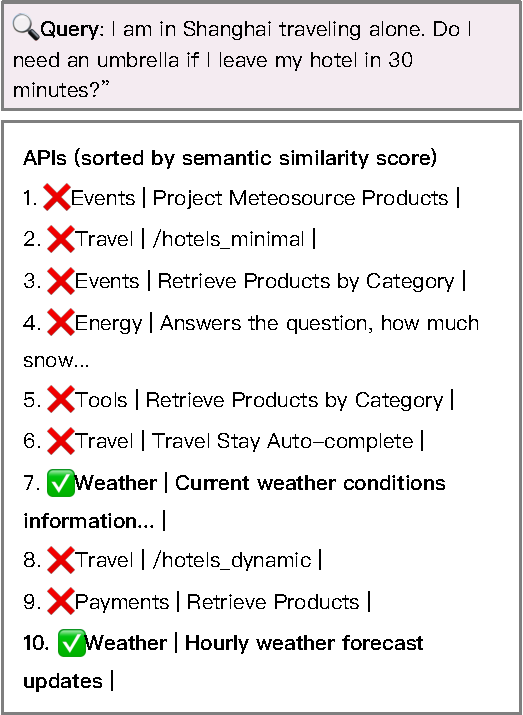
\includegraphics[height=8cm]{../assets/ch3-为何需要微调.pdf}
  \bicaption{使用开源向量模型得到的工具排序结果}{工具 Ranking Using Open-source Embedding Models}
  \label{fig:why-tune}
\end{figure}

因此,为了解决上述问题,本文提出了基于通用向量模型进行微调,通过构造高质量的工具训练数据来将领域知识注入模型,从而提升模型在工具选择上的准确性。

在训练向量模型时,训练数据包含三个部分:正样本,负样本,查询语句。
查询语句即为数据集中的“query”字段,对应用户输入的查询信息。
正样本也可以直接使用数据集提供的参考工具列表。

对于负样本的部分,如图~\ref{fig:negative-sample-generation},我们采取了两种不同的负样本构造方式:
一种是简单负样本(Simple Negative)构造,另一种是困难负样本构造(Hard Negative)。

\begin{figure}[!htp]
  \vspace{1em}
  \centering
  \setlength{\abovecaptionskip}{10pt} % 控制图片和caption之间的距离
  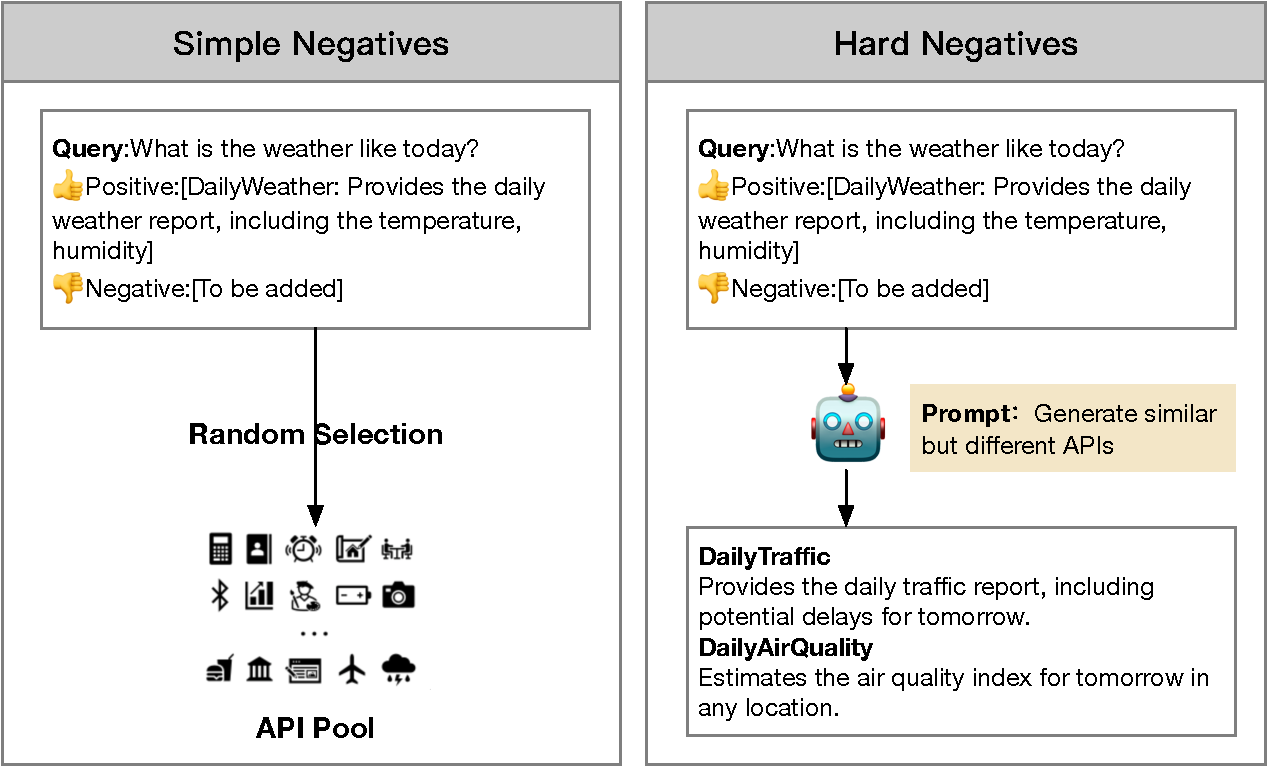
\includegraphics[height=7cm]{../assets/ch3-负样本构造.pdf}
  \bicaption{负样本构造的两种方式}{Negative Sample Generation}
  \label{fig:negative-sample-generation}
\end{figure}

\indent \textbf{简单负样本构造}。对于简单负样本构造,我们直接选择不同类别的K个工具作为负样本。
在简单负样本构造中,不同类别的工具之间的功能上一般有区别,因此简单负样本构造能够保证负样本与正样本之间在工具上的差异。

\indent \textbf{困难负样本构造}。在工具选择、调用场景,开源的通用向量模型难以区分工具之间细微的语义区别。
困难负样本构造的目的是帮助模型更好地区分工具之间细微的语义区别,帮助更好地应对噪声。
我们选择采用GPT-3.5完成困难负样本的构造。由于原工具数据量众多,
从中筛选语义表述类似、但是功能上有区别的工具样本费时费力。
因此我们采取了直接用大语言模型生成工具描述作为负样本的策略。

具体策略如下:
首先,我们采样一批<query,推荐工具>的数据,
然后我们通过提示词将用户需求和工具描述提供给大语言模型,
要求模型生成类似但是功能上无法满足用户需求的工具描述。
通过这样遍历工具描述生成负样本,可以生成一组高质量的困难负样本供模型学习。

\subsubsection{自我反思机制}

自我反思机制的主要目的是对生成的工具调用路径进行反思,以提升整体的准确率。

自我反思机制的触发时间点有三个:1.动态寻路算法找到路径并主动结束路径
2.动态寻路算法超过了最大迭代次数并终止或放弃寻路

具体而言,自我反思模块的输入是
我们当前的工具调用路径和用户需求,
根据工具召回器召回的初始节点,
以及我们撰写的反思格式说明。
输出包括以下几部分:1.成功/部分失败/完全失败的等级
2.若部分失败,从哪一个工具节点开始为首个错误节点 3.若全部失败,有哪些可以删除的噪声工具初始节点

评价为“成功”的路径,我们直接进入工具调用模块进行调用。
对于评价为“失败”的路径,我们
会根据失败的等级选择进行不同的重新寻找工具调用路径:
第一种是从中间步骤开始重新寻找路径,
另一种是从头开始重新寻找路径。

\begin{enumerate}
  \item \textbf{从中间步骤继续}: 在任务未完成的情况下,
  我们将在短期记忆中记录寻路过程中的每一步的选择节点和理由。
  当路径被标记为“放弃”或被评判器认定为“失败”时,我们会重新激活该路径上的智能体,
  并将识别到的失败原因重新纳入历史上下文。
  评判器在判定“失败”时,通常会标记出它认为的第一个出现错误的节点。
  在重新激活智能体并进行寻路时,我们将从该节点继续,
  而不是从头开始。这种从中间步骤继续的策略不仅能够加快寻路速度,
  减少大语言模型的调用次数,还能充分利用先前成功调用的经验,
  从而提升决策的准确性。
  \item \textbf{重新寻路}: 在自我反思模块认为路径“完全失败”时,
  我们需要从头开始重新生成整条路径。评判器会识别路径初始节点中与用户查询无关的工具名称作为反思的一部分。
  为了提高系统的整体效率,我们会首先从初始工具节点中移除这些无关的工具,
  避免大模型受到这些噪声的影响,从而选择无关的工具进行调用,
  导致后续调用出错。通过这一清理过程,我们能够有效减少噪声工具的影响,
  确保后续搜索的准确性。\par
  接下来,我们将会在经过噪声清理的工具组中重新开始选择下一节点并组成路径。
  这种从头开始的自我反思允许算法在一个更加简洁与优化的初始条件下进行搜索,
  从而提升工具调用路径的质量与响应速度。
\end{enumerate}
 
该自我反思机制可以反复应用,直至满足终止条件为止。这种持续的反思过程确保了对问题的逐步优化,
有助于形成更加有效的调用路径。

综上所述,这两种反思策略——从中间步骤继续优化和从头开始的寻路——的结合使用,
能够在处理用户需求未满足的情况下,提供更高的灵活性与效率。
通过不断的反思与优化,系统将逐步提升其在动态环境中的适应能力,确保用户体验的持续改进。

\subsubsection{工具调用路径记忆框架}

本节提出了一种增强模型规划和推理能力的记忆框架,该框架分为短期记忆和长期记忆两个部分。短期记忆聚焦于动态推理过程中的实时信息记录,长期记忆则存储历史调用路径以支持未来推理任务的优化。

\paragraph{短期记忆}

短期记忆是模型在图上动态推理时保存的状态信息,旨在实时支持当前推理过程。其内容包括用户任务、当前遍历节点、历史遍历节点以及调用路径等关键数据。在推理过程中,短期记忆会被动态更新,以反映当前状态和推理环境。为确保模型能够感知这些状态信息,我们将短期记忆存储于内存中,并在每次推理时通过构建提示词直接将其注入大语言模型的上下文。这种机制不仅能帮助模型理解当前推理场景,还能提高其规划和决策的准确性。

\paragraph{长期记忆}

长期记忆用于存储历史工具调用路径及其对应的推理结果,并随着调用次数的增加不断扩展。这些信息存储在数据库中,并在后续推理任务中通过相似度检索为模型提供支持。长期记忆的核心目标是利用历史经验优化模型的规划与工具选择能力。

长期记忆模块基于检索增强生成(Retrieval-Augmented Generation, RAG)框架,将历史上成功的 \textless 子任务描述, 工具调用路径\textgreater\ 转化为向量存储。对于新的任务需求,系统会将其嵌入为向量,并与长期记忆库中的向量进行相似度计算。通过排序,系统检索出与当前需求最相似的 \(K\) 个历史任务及其工具调用路径。最终,这些历史任务的调用路径和描述以自然语言的形式被注入大语言模型的上下文,作为提示词辅助工具选择模块的推理与执行。

这种结合短期与长期记忆的框架,既能动态适应实时推理的需求,又能通过历史知识积累,增强模型对复杂任务的规划能力,从而显著提高系统的效率与准确性。

\subsection{工具调用与总结模块}
\label{sec:real_tool_simulation}

\subsubsection{整体逻辑}

工具调用模块的主要功能是执行规划好的工具调用DAG,并将得到的结果返回给系统,
从而为后续的推理和规划提供支持,最终调用LLM来进行总结,生成符合用户需求的答案。

工具调用部分的整体逻辑可以分为两个主要部分:工具调用和工具响应解析。
具体而言,我们首先根据工具的描述信息和用户需求生成工具调用的参数,
然后通过代码生成请求体并通过工具调用接口将请求体发送给目标工具,
以获取其响应。
获得响应后,理论上我们可以直接将所有工具的调用结果直接提供给总结器,要求模型根据工具响应输出最终结果。
在系统设计中,为了方便流程的管理和设计,我们将工具总结智能体作为一种特殊的工具,在所有工具都执行完毕之后,
调用该工具对其他工具响应结果进行总结和输出,作为系统的最终输出。

但由于每个响应的长度参差不齐,对于一些响应长度较长的工具,
可能单个工具的响应数据就超出了大语言模型的上下文限制。
因此,我们添加了一个基于大语言模型的响应压缩模块,
通过对响应的压缩来缓解大语言模型的上下文限制,以便于工具参数生成和工具总结器的正确执行。

\subsubsection{工具并行调用模块}

工具并行调用模块的目标是优化工具调用DAG的执行效率,特别是在多个工具之间没有依赖关系的情况下,通过并行处理显著缩短整体运行时间。

\paragraph{并行调用逻辑}

在工具调用DAG中,每个工具节点可能存在两种关系:
\begin{enumerate}
    \item 独立节点:工具之间无参数或时序依赖,可同时执行。
    \item 依赖节点:工具的输入参数依赖于其他工具的输出,必须按照依赖关系依次执行。
\end{enumerate}

为了实现并行调用,我们首先对工具调用DAG进行拓扑排序,以明确工具的依赖关系。然后根据以下步骤划分工具调用组:
\begin{enumerate}
    \item 将无前序依赖的工具分组为一个批次,并行启动调用。
    \item 等待当前批次所有工具完成后,获取其输出结果并解析。
    \item 将当前批次的输出作为后续工具的入参,继续处理下一批次工具。
\end{enumerate}

这种逻辑确保了工具的调用顺序既满足依赖关系,又尽可能实现并行化处理,从而提高整体执行效率。如图\ref{fig:parallel-invocation-logic}所示,

\begin{figure}[!htp]
  \centering
  \setlength{\abovecaptionskip}{10pt}
  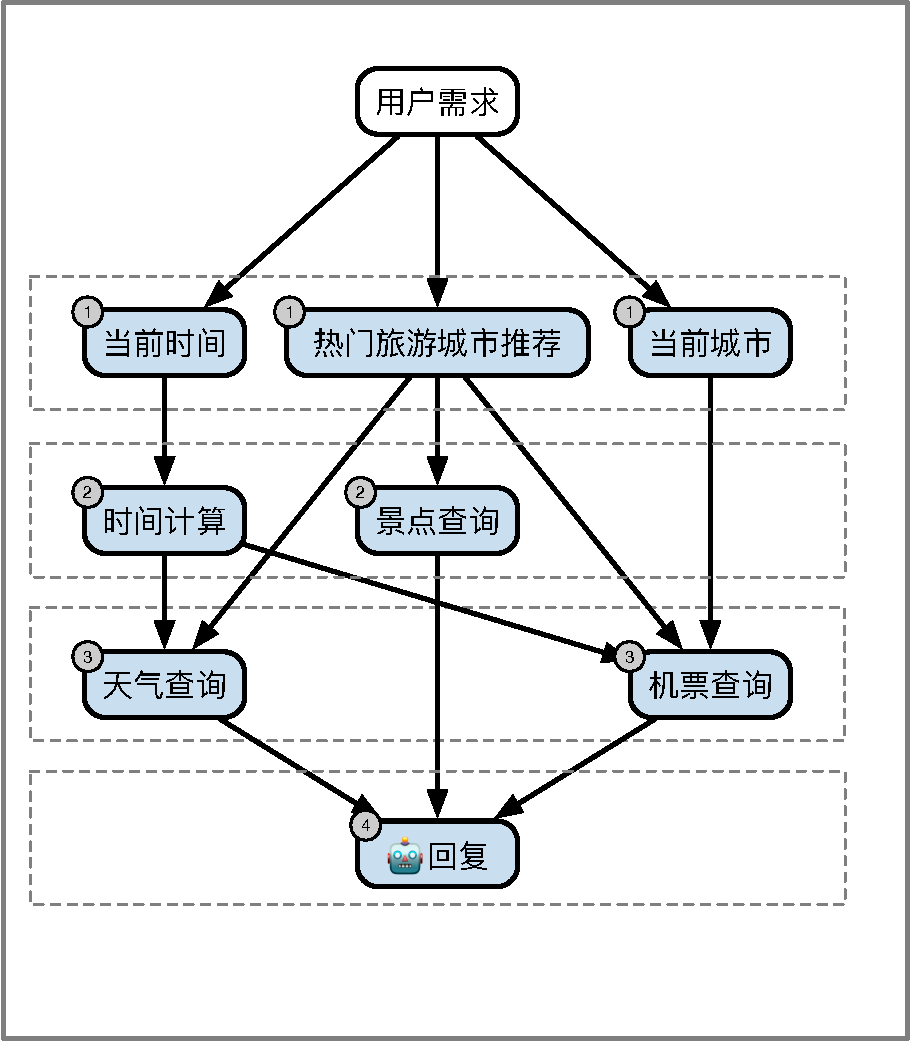
\includegraphics[height=8cm]{../assets/ch4-并行调用模块.pdf}
  \caption{工具并行调用逻辑}
  \label{fig:parallel-invocation-logic}
\end{figure}

工具并行调用的主要优势包括以下三个方面:首先,通过将无依赖关系的工具分阶段并行启动,避免了工具调用之间的相互阻塞,显著提高了整体处理效率;其次,并行逻辑优先优化关键路径的工具调用时间,同时使独立路径上的工具可以并行完成,从而有效缓解关键路径的瓶颈问题,减少关键路径上的总耗时;最后,并行调用支持多个工具同时调用大语言模型(LLM)进行处理,降低因串行调用而累计的LLM响应延迟,大幅提升系统的整体运行效率。

\paragraph{时间复杂度与性能分析}

假设工具调用DAG包含 \(x\) 个工具,其中每个工具的平均调用耗时为 \(t\),最长依赖路径包含 \(L\) 个工具节点。则顺序调用的总耗时为:
\[
T_{\text{顺序}} = \sum_{i=1}^{x} t_i \approx x \cdot t
\]
而并行调用的总耗时由最长依赖路径 \(L\) 决定:
\[
T_{\text{并行}} = \sum_{i=1}^{L} t_i \approx L \cdot t
\]

在无依赖情况下,所有工具均可并行调用,此时整体耗时仅为单个工具中耗时最长的调用时间:
\[
T_{\text{无依赖并行}} = \max_{i=1}^{x} t_i
\]

然而,在实际应用中,工具调用的总时间还需考虑 LLM 的延迟因素:
\[
T_{\text{实际}} = T_{\text{工具调用}} + T_{\text{LLM延迟}}
\]
其中:
\begin{itemize}
    \item \(T_{\text{工具调用}}\) 是工具执行的时间,由上述拓扑排序及并行调用决定。
    \item \(T_{\text{LLM延迟}}\) 包括请求体生成时间与响应压缩时间,具体取决于工具数量和响应数据的规模。
\end{itemize}

以一个具体的示例说明:假设工具调用DAG有 10 个工具,每个工具的平均调用耗时为 \(t = 1 \, \text{秒}\),最长依赖路径包含 4 个节点(\(L = 4\))。如果顺序调用,总耗时为:
\[
T_{\text{顺序}} = 10 \cdot 1 = 10 \, \text{秒}
\]
而通过并行调用,总耗时降至:
\[
T_{\text{并行}} = 4 \cdot 1 = 4 \, \text{秒}
\]
实际系统中需加上 LLM 的延迟时间,但并行调用的节省逻辑依然成立,尤其在依赖关系较少或任务分布均匀的情况下。

并行调用通过优化工具的执行顺序,有效缓解了因依赖关系导致的等待时间长的问题。尽管 LLM 的生成延迟和响应压缩带来额外时间开销,但并行逻辑依然能够充分利用资源,显著提升系统的整体效率。

\subsubsection{工具入参生成模块}

工具入参生成模块的主要任务是为工具调用动态生成请求体。请求体中固定的信息(如请求URL、请求方式、Key等)可以从工具图谱和配置文件中直接获取,而动态生成部分主要包括工具的请求参数列表。

根据工具调用的流程,每个工具可能存在零到多个前序工具,这些前序工具的输出可能会直接影响当前工具的参数生成。

为了正确生成当前工具的入参,系统在所有前序工具调用完成后,会将以下信息提供给参数生成智能体:当前工具的名称和描述、参数列表及其描述、前序工具的调用响应以及参考格式。

随后,系统会对生成的JSON字符串进行解析,得到实际的JSON对象作为参数。解析后的参数需要经过严格校验,以确保其符合预期要求。校验内容包括三个方面:一是\textbf{参数完整性},验证是否缺少必选参数;二是\textbf{参数类型},确保每个参数的类型(如整数、字符串、数组)与定义一致;三是\textbf{参数名称},检查生成的参数名称是否与工具的参数定义匹配。校验过程可以形式化表示为:
\[
\text{validate}(P_{\text{parsed}}) =
\begin{cases}
\text{True}, & \text{若参数满足所有校验规则;} \\
\text{False}, & \text{若参数校验失败。}
\end{cases}
\]

若校验未通过,系统将返回固定的错误信息,并要求参数解析器重新生成参数。这一过程会循环执行,直到满足以下条件之一:参数生成成功且通过校验,或者达到最大尝试次数,系统放弃当前工具的调用。

当参数生成成功并通过校验后,系统会调用固定的函数来执行工具请求。工具调用的响应通常以JSON格式返回,随后会被提供给响应解析模块,进行进一步的处理和利用。

通过结合工具依赖关系、大语言模型生成能力和严格的参数校验机制,工具入参生成模块能够确保工具调用请求的准确性和鲁棒性,同时提高整体系统的可靠性。

\subsubsection{工具响应解析模块}

生成请求体后,我们通过工具调用接口将其发送给目标工具,并获取对应的响应数据。工具的响应数据通常以JSON格式返回,其中可能包含大量信息。然而,这些信息并不总是直接相关。通过实验分析发现,许多工具的返回内容中包含冗余信息,这使得响应数据长度过长,难以直接输入到大语言模型中进行处理。直接依赖大语言模型从中提取重要信息在某些情况下会导致效率下降。因此,我们引入了响应压缩模块,旨在尽可能保留关键信息的同时减少响应数据的长度,使其能够更高效地适配大语言模型的上下文限制。

由于工具响应的格式通常不固定,难以预先确定哪些字段应保留或舍弃,因此我们采用大语言模型分析工具响应的示例,仅保留与用户需求相关的字段,从而减小响应长度。

如图~\ref{fig:ch4-compression} 所示,响应压缩模块的逻辑流程如下:

\begin{figure}[!htp]
  \vspace{1em}
  \centering
  \setlength{\abovecaptionskip}{10pt} % 控制图片和caption之间的距离
  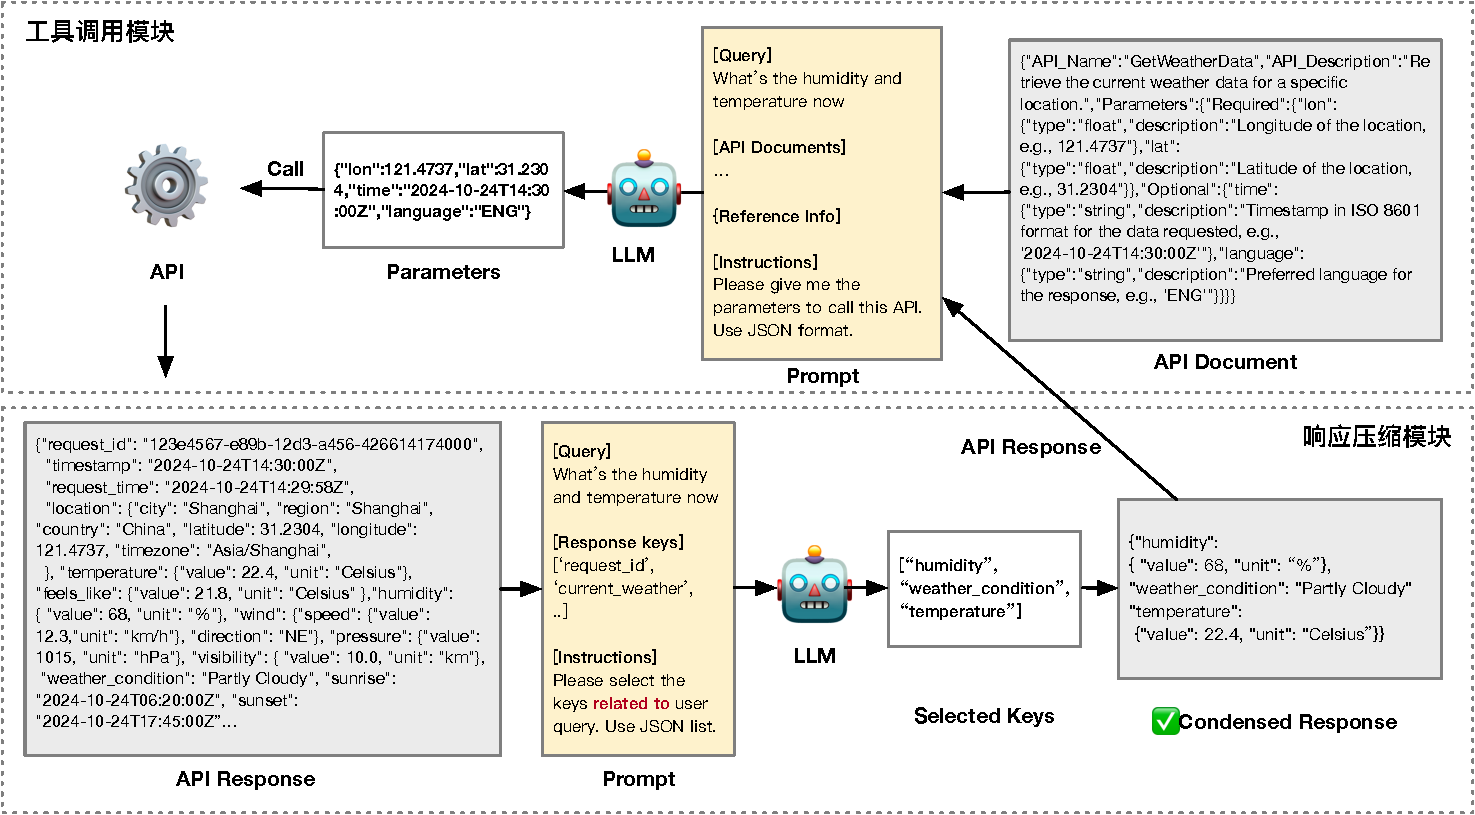
\includegraphics[height=7cm]{../assets/ch4-工具调用模块.pdf}
  \bicaption{响应压缩模块}{Compression of API responses}
  \label{fig:ch4-compression}
\end{figure}

响应压缩的流程可以分为以下三个阶段:

首先,\textbf{提取工具文档信息}。所有工具均来自ToolBench等开源数据集,这些数据集包含每个工具的详细描述和示例响应信息。我们将工具名称、功能描述、参数信息以及工具响应示例作为文本输入大语言模型。这些信息构成了压缩模块的基本提示词。

其次,\textbf{生成压缩提示词}。我们为大语言模型提供详细的规则,要求模型根据工具的功能描述提取最相关的信息。例如,工具版本、调用时间以及无效信息等与实际功能无关的内容会被舍弃,而关键字段将被保留。

最后,\textbf{添加上下文学习示例}进行强化提示。我们选取三个上下文学习示例,每个示例包含一个原始响应和对应的专家撰写的压缩响应。通过这些示例,我们要求压缩器以自然语言输出保留的字段,并使用正则表达式匹配生成字段列表,最终用代码逻辑筛选出需要的字段及其内容。

在实际应用中,当工具响应长度超过1024个字符时,系统会优先移除不重要的信息进行压缩。如果压缩后仍然超过1024个字符,则进一步截取压缩结果的前1024个字符。这种方法有效减少了工具响应的长度,避免冗余信息的干扰,并缓解了大语言模型上下文窗口的限制,从而确保系统调用的正常运行。

% 通过对ToolBench数据集的分析,工具的平均响应字符串长度为\textit{xxx}个字符。经过响应压缩后,最长的响应也不超过1024个字符,总体上减少了超出上下文限制的情况\textit{xx\%},并且平均每个工具响应节省了\textit{xx}个字符。这种方法在提升系统效率和响应适配性方面效果显著。

\subsubsection{工具总结器}

在所有的工具都调用完毕之后,我们通过调用工具总结器对工具的调用结果进行总结,以生成符合用户需求的答案。
工具总结器并不会获取所有工具的响应,而是会根据在子任务分解时的依赖关系选择部分工具的响应结果来进行总结,即仅选择与回答有直接关联的工具响应。


这部分方法的设计类似于传统的检索增强生成(Retrieval-Augmented Generation, RAG)。在这里,通过工具调用得到的结果可以看作是类似于检索阶段的信息,而基于这些结果生成对用户需求的回答则对应于生成阶段。在这一框架中,核心目标包括:1)减少幻觉现象,确保生成的内容基于真实信息;2)确保回答的稳定性,即相同的输入能够生成一致的答案;3)提升回答的相关性,降低无关信息(噪声)的干扰。

为实现上述目标,我们设计了一个用于工具总结模块的提示词模板,通过提示词工程引导模型生成回答。如下所示,该模板为模型提供了一种结构化的思考和表达方式,使得生成的内容更加稳定、有逻辑,并能够准确满足用户的需求,从而有效提升生成质量。

% Set Colors
\definecolor{bgcolor}{RGB}{240,240,240} % Background color
\definecolor{titlecolor}{RGB}{20,20,20} % Title background color

\begin{center}
% Create background with tcolorbox
\begin{tcolorbox}[colback=bgcolor, colframe=black, width=0.85\textwidth, boxrule=0.5mm, 
coltitle=white, colbacktitle=titlecolor, title=An Example for Response Generation with GPT-4]

% Centered content

\textbf{Instruction Prompt:} Generate a response to the user's question based on the results from the tools and your internal knowledge.

\textbf{Task:} What's the most popular travel destination in Europe? And what's the weather like there?

\textbf{Return from Tool Calling:} 
\{%
    "popular\_travel\_destination": \{%
        "destination": "Paris, France",%
        "popularity\_score": 9.8%
    \},%
    "global\_weather\_search": \{%
        "location": "Paris, France",%
        "weather": \{%
            "temperature": "15°C",%
            "condition": "Partly Cloudy",%
            "humidity": "60\%",%
        \},%
        "timestamp": "2024-11-17T14:00:00Z"%
    \}%
\}

\textbf{Instructions:}
1. If the tool's output is incorrect, or if the information from the tools and your internal knowledge is insufficient to answer, do not respond. Avoid fabricating any untrue information.

2. Think step by step before answering. Plan the key points to address before formulating your response.

3. Only answer the user's request. Do not include any additional or irrelevant information.

4. Use the same language as the Task (in this case, English).

5. Provide the output in JSON format.

\textbf{Output Format:}  
\{%
    "Steps": [%
        "Find the most popular travel destination in Europe.",%
        "Describe the current weather at that destination."%
    ],%
    "Result": "The most popular travel destination in Europe is Paris, France. The weather in Paris is partly cloudy with a temperature of 15°C, a humidity level of 60\%."%
\}

\end{tcolorbox}
\end{center}

\section{本章小结}
\label{sec:summary_chap4}

本章提出了一种基于工具图谱和深度优先遍历的动态工具编排与调用方法,通过任务分解模块将复杂需求拆解为子任务,并利用深度优先遍历算法动态规划工具调用路径,以应对工具动态性和复杂依赖关系。结合记忆框架,有效利用历史经验优化路径选择效率,同时通过语义相似度优化的工具召回器提升工具选择的准确性。工具调用模块支持并行处理和响应压缩,减少大语言模型的上下文压力,提高执行效率。最终,通过工具总结模块对调用结果进行整合与回答生成,确保输出的准确性和相关性。本方法有效结合了工具图谱的结构化信息与大语言模型的动态决策能力,为复杂任务的灵活、高效、精准解决提供了系统化的支持。